%However, the picture painted by these findings might be misleading. First of all, there is a possibly confounding factor. Contrast, from Experiment 1, an expression from the vague condition: `the square with few dots' with an expression from the crisp condition: `the square with 5 dots'. One difference is that `few' has the potential for vagueness, whereas `5' is crisp. But another difference is that `few' is verbal while `5' is numerical, in the sense that a number is mentioned explicitly. Since these two differences could not be separated in Experiment 1, the vagueness advantage finding is vulnerable to an alternative interpretation, that what we saw as a vagueness advantage was in contrast an advantage for the verbal form of the quantifier. In Experiment 2 we therefore created verbal and numeric versions of each of the vague and crisp instructions so that we could compare vague and crisp conditions while taking account of verbal / numeric format.

%Another potential problem with Experiment 1 is the following. Participants chose one of two squares: therefore the `vague' quantifiers (e.g., `few') uniquely identified one square. Recall our definition of vague  -- ``a word is precise if it describes a well-defined set of objects. By contrast, a word is vague if it is not precise''.  In Experiment 1, the quantifiers in the vague conditions did not realise their potential for vagueness. This is because there were no borderline cases of the referent that could make the referent set `not well-defined', and perhaps because using definite articles in the instructions implied that only one option was correct. Using error feedback in Experiment 1 could have exacerbated this.

To find out what happens when words are used in a context where their potential for vagueness comes to the fore, Experiment 2 used three arrays (rather than two) so that the vague description had more than one possible referent, and used indefinite articles to avoid the impression that only one response counted as correct, and was carried out without error feedback.
An indication that the potential for vagueness was realised in Experiment 2 is that the borderline response was chosen fairly often: 16\% of the time.

In Experiment 2, an item was a referring expression instruction followed by a set of three dot arrays defined by a triple of numbers, representing the number of dots in the left, middle, and right arrays. We used four different triples of numbers: (6,15,24); (16,25,34); (26,35,44); (36,45,54). Each set of arrays comprised three arrays (instead of two as in Experiment 1); the array representing the central number was always presented in the middle of the three; there were two flanking arrays where one had fewer dots than the central array and the other had more.

Examples of crisp and vague versions of the numerical and verbal instructions follow: the examples assume the array (6,15,24) and reference to the smaller number of dots, such that 6 was classified as the expected response; 15 as the borderline response; and 24 as the incorrect response. In the {\em vague numerical} condition we used \emph{Choose a square with about 10 dots}. None of the squares contained 10 dots. 10 is slightly closer to 6 than to 15, justifying 6 as the best response and 15 as the borderline response. In the {\em vague verbal} condition we used \emph{Choose a square with few dots}. In the {\em crisp numerical} condition we used \emph{Choose the square with 6 dots}, and one square always did contain the number mentioned. For {\em crisp verbal}, we used \emph{Choose the square with the fewest dots}.

\begin{table}
\centering
\caption{Experiment 1 instructions arranged by condition. The instructions given in the table started with ``Choose \ldots"}
\label{instructionse2}
\begin{tabular}{cccll}
\hline\noalign{\smallskip}
Item & Quantity & Number & Crisp & Vague\\
\noalign{\smallskip}\hline\noalign{\smallskip}
06:15:24 & Small & Numeric & the square with 6 dots & a square with about 10 dots\\
06:15:24 & Small & Verbal & the square with the fewest dots & a square with few dots\\
06:15:24 & Large & Numeric & the square with 24 dots & a square with about 20 dots\\
06:15:24 & Large & Verbal & the square with the most dots & a square with many dots\\
\noalign{\smallskip}\hline\noalign{\smallskip}
16:25:34 & Small & Numeric & the square with 16 dots & a square with about 20 dots\\
16:25:34 & Small & Verbal & the square with the fewest dots & a square with few dots\\
16:25:34 & Large & Numeric & the square with 34 dots & a square with about 30 dots\\
16:25:34 & Large & Verbal & the square with the most dots & a square with many dots\\
\noalign{\smallskip}\hline\noalign{\smallskip}
26:35:44 & Small & Numeric & the square with 26 dots & a square with about 30 dots\\
26:35:44 & Small & Verbal & the square with the fewest dots & a square with few dots\\
26:35:44 & Large & Numeric & the square with 44 dots & a square with about 40 dots\\
26:35:44 & Large & Verbal & the square with the most dots & a square with many dots\\
\noalign{\smallskip}\hline\noalign{\smallskip}
36:45:54 & Small & Numeric & the square with 36 dots & a square with about 40 dots\\
36:45:54 & Small & Verbal & the square with the fewest dots & a square with few dots\\
36:45:54 & Large & Numeric & the square with 54 dots & a square with about 50 dots\\
36:45:54 & Large & Verbal & the square with the most dots & a square with many dots\\
\noalign{\smallskip}\hline
\end{tabular}
\end{table}

\subsection{Hypotheses} 

We formulated the following hypotheses for Experiment 2:

\begin{description}
	\item [Hypothesis 1] There exists a main effect RT advantage for vagueness.
	\item [Hypothesis 2] An RT advantage for vagueness both in \emph{numeric} and in \emph{verbal} instructions.
	\item [Hypothesis 3] No large main effect of instruction format (i.e., numeric versus verbal) since we hypothesised that vagueness rather than instruction format drove the effect in Experiment 1.
	\item [Hypothesis 4] On the basis of Experiment 1, we expect faster responses for stimuli with more discriminable arrays.(i.e., an effect of item).
	\item [Hypothesis 5] Participants should make more borderline case choices for vague than crisp instructions.
\end{description}

\subsection{Experimental Method} 

% Participants were aged between 18 and 45 with a median age of 28. 
We manipulated as independent variables vagueness and instruction format (i.e., numeric versus verbal instructions), yielding four conditions, \emph{vague numeric}; \emph{vague verbal}; \emph{crisp numeric}; \emph{crisp verbal}.
We measured two dependent variables: response time; and the probability of a participant choosing the borderline case.
On each trial, first the referring expression that constituted the instruction for that trial was displayed. 
Participants then pressed a key to indicate that they had read the instruction. 
After 1000 ms, the arrays were presented, while preserving the text of the referring expression. 
The response time dependent variable was measured from the presentation of the arrays, until the keypress indicating the participant's choice, which was also recorded. 
The trial would timeout after 60 seconds if there was no response.
In this experiment, no feedback was given. 
This was because, in the vague conditions, we did not regard any response as `correct' or `incorrect', but instead as `borderline response', or `not borderline response', and we did not want to draw participants' attention to this distinction explicitly. 
We simply recorded whether the participant chose the best referent, the borderline case or the poorest referent, and how long it took the participant to respond.

\subsection{Results} 

Means for response times and proportion of borderline responses are given in Fig. (\ref{resultse2}). 
Response times from all trials were trimmed at 2.5 standard deviations for each subject, leading to the loss of 236 trials, 3.1\% of the data. 
A linear mixed model was constructed for the (logged) response times, 
with sum-coded vagueness, instruction format, (and their interaction), and item as fixed effects, and the same effects as slopes over participant for random effects. We found:

\begin{description}
	\item [Test of Hypothesis 1] The main effect of \emph{vagueness} was to slow responses down, in contrast with Experiment 1, and offering evidence against Hypothesis 1 (vague: 2668 ms; crisp: 2450 ms; a difference of 218 ms; $\beta=.06$, $se=.01$, $t=4.6$, $p<0.0001$). 
	\item [Test of Hypothesis 2] In focussed comparisons, vagueness was significantly disadvantageous in the \emph{numeric} conditions ($\beta=0.09$, $se=0.02$, $t=4.5$, $p<0.0001$), and non-significantly disadvantageous in the \emph{verbal} conditions ($\beta=0.02$, $se=0.02$, $t=1.5$, $p=0.1550$), offering partial evidence against Hypothesis 2. The disadvantage for vagueness was greater in the numerical than in the verbal conditions, leading to a significant overall interaction effect between vagueness and instruction format ($\beta=-0.13$, $se=0.02$, $t=-6.6$, $p=0.0169$).
	\item [Test of Hypothesis 3] There was a significant effect of \emph{instruction format} with numerical conditions attracting longer responses than the verbal conditions: consistent with Experiment 1, but suggesting that instruction format rather than vagueness drove the effect we observed in Experiment 1 (numeric: 3284 ms; verbal 1866 ms; a difference of 1418 ms; ($\beta=-0.36$, $se=0.07$, $t=-5.1$, $p<0.0001$).
	\item [Test of Hypothesis 4] There was a significant main effect of item (i.e., of which triple of numbers of dots were used in the stimulus): ($\beta=0.12$, $se=0.02$, $t=7.1$, $p<0.0001$). This effect seems likely to be due to the very fast responses for stimuli using arrangements of the smallest numbers of dots (6,15,24), which also had the largest difference in ratio of smallest number to largest number in the stimulus, suggesting that stimuli using these numbers of dots may have been particularly discriminable for participants.
\end{description}

A generalized linear mixed model \citet{jaeger2008categorical} was fit to the data for selection of the borderline response, with sum-coded vagueness, instruction format, (and their interaction), and item as fixed effects, and the same effects as slopes over participant for random effects. The distribution of responses over the nearest match square, the borderline square, and the furthest match square are given in Fig, \ref{resultse2}. Participants chose the borderline square on $16.6\%$ of trials overall.

\begin{description}
	\item [Test of Hypothesis 5] Participants were significantly more likely to choose the borderline option for vague instructions than for crisp instructions (21.9\% vs 11.3\%: $\beta=0.62$, $se=0.22$, $z=2.8$, $p=0.0059$). Participants were also significantly more likely to choose the borderline square when the instruction used the numerical format rather than the verbal format (30.1\% vs 3.0\%: $\beta=-3.35$, $se=0.23$, $z=-14.6$, $p<0.0001$). 
\end{description}

\begin{figure}[htbp]
\centering
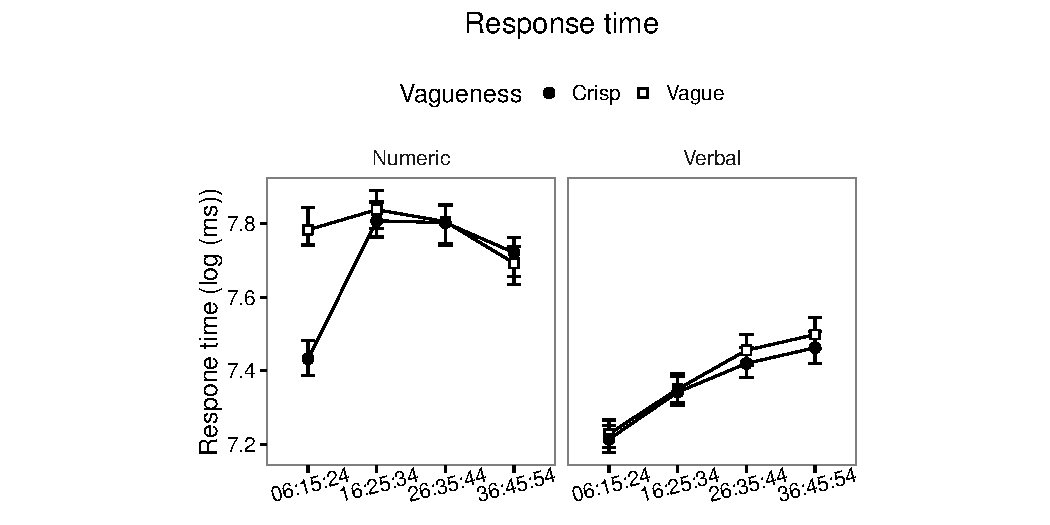
\includegraphics[trim = 20mm 0mm 35mm 0mm, clip, width=.49\textwidth]{figures/e2-rtplot-1.pdf}
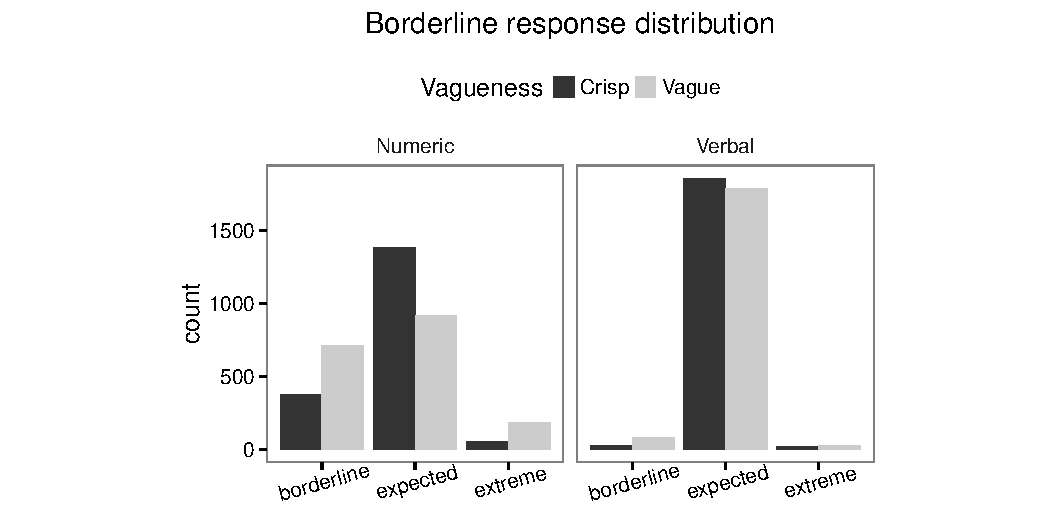
\includegraphics[trim = 20mm 0mm 35mm 0mm, clip, width=.49\textwidth]{figures/e2-blBarChart-1}
\caption{Experiment 2 results: mean response times by condition and item, and counts of borderline case responses by condition.}
\label{resultse2}
\end{figure}

\subsection{Discussion}

Experiment 2 tested to see whether when borderline cases are present, vague instructions would speed responses as they did in Experiment 1 when there were no borderline squares. 
We actually found a small (but statistically significant) \emph{disadvantage} of vague instructions: vague instructions slowed people down by 112 ms on average. We also found that the effect of instruction format was significant, with numerical format slowing responses by 689 ms on average, such that the disadvantage of numerical format overwhelmed the contribution of vagueness. The \emph{verbal vague} condition was still responded to faster than the \emph{numerical crisp} condition, so the pattern from Experiment 1 was reproduced, but in the light of the evidence from Experiment 2, in the presence of borderline cases, the advantage that was ascribed to vagueness before now looks more like an advantage of verbal instruction format.

However, once again there is a possibly confounding factor. Observe that, in Experiment 2, instruction format (i.e., the choice between numeric and verbal) went hand in hand with might be called the (human) {\bf selection algorithm}: To see this, consider the task of selecting the dot array that contains ``few dots'': to do this, it suffices to {\em compare} the three arrays and select the one that contains the fewest elements.  To select the dot array that contains ``16 dots'' seems to require the participant to estimate, and then {\em match}, the cardinality of (at least) one dot array to 16, a process which could plausibly take longer, independently of vagueness. Therefore, our results so far permit the interpretation that what made the instructions in the verbal condition fast is not the fact that they were worded verbally, but that they allowed participants to use a comparison ``algorithm''.

In the next two experiments we pitted the comparison algorithm and matching algorithm selection tasks against each other while controlling vagueness and instruction format. In Experiment 3 we restricted all the instructions to \emph{numeric} quantifiers while factorially manipulating vagueness and selection task. In Experiment 4 we ensured that all instructions used \emph{verbal} quantifiers, while also factorially manipulating vagueness and selection task. This allowed us to distinguish between the predictions of the selection task account and the instruction format account. 
